\documentclass[12pt,a4paper,twoside,openright,fleqn]{mwrep}
\usepackage[latin2]{inputenc}
\usepackage[OT4,plmath]{polski}
\usepackage{amsmath}
\usepackage{amssymb}
\usepackage{graphicx}
%\usepackage[a4paper,left=3.5cm,right=2.5cm,top=2.5cm,bottom=2.5cm]{geometry}
\usepackage[width=16cm,height=25cm]{geometry}
\usepackage{fancyvrb}
\usepackage{listings}
%\usepackage{bold-extra}
\usepackage[unicode=true]{hyperref}
\usepackage{color}
\usepackage{cite}
\usepackage{float}

\pagestyle{uheadings}

% Definicje ustalaj�ce wygl�d wydruk�w program�w
\definecolor{darkgray}{rgb}{0.95,0.95,0.95}
\lstset{frame=tb, backgroundcolor=\color{darkgray}}
\lstset{numbers=left, numberstyle=\tiny, stepnumber=2, numbersep=5pt}
\lstset{basicstyle=\ttfamily\footnotesize, keywordstyle=\color{blue}\bfseries}
\lstset{tabsize=2}


\hypersetup{
    pdfpagemode=UseOutlines,   % otwiera dokument w trybie jednej strony
    pdfpagelayout=SinglePage,  %
    pdfstartpage=1,            % na podanej stronie
    bookmarksopen=true,        % rozwini�cie zak�adek
    bookmarksopenlevel=1,   % do jakiego poziomu
    colorlinks=true,   % kolorowanie odno�nik�w zamiast ramki wok� nich
    citecolor=cyan,   % kolor odno�nik�w do bibliografii, domy�lnie zielony
    filecolor=red,   % kolor odno�nik�w do lokalnych plik�w, domy�nie magenta
    linkcolor=blue,   % kolor odno�nik�w wewn�trznych, domy�lnie czerwony
    menucolor=green,   % kolor pozycji menu Acrobata, domy�lnie czerwony
    urlcolor=blue,   % kolor odno�nik�w do adres�w internetowych, domy�lnie cyan
                               % DANE DOKUMENTACJI
    pdfauthor={ARR2016},
    pdftitle={Projekt przej�ciowy --- Symulator laboratorium L1.5},
 }
                                   % DEFINICJE W�ASNE
\newcommand{\dd}{\text{d}}
\newtheorem{uwaga}{Uwaga}
\newtheorem{twr}{Twierdzenie}

\title{Projekt przej�ciowy --- Symulator laboratorium L1.5}
\author{ARR 2016}
\date{\today}


\begin{document}
\VerbatimFootnotes

\maketitle
\tableofcontents

\chapter{Wst�p}

\section{Motywacja}

Projekt wirtualnego laboratorium powsta� jako pomoc dydaktyczna do zaj�� laboratoryjnych wykonywanych na robotach Pioneer w �rodowisku ROS realizowanych na Politechnice Wroc�awskiej. Dzi�ki �rodowisku studenci mog� w ramach przygotowania do zaj�� wykona� �wiczenia na robotach Pioneer w systemie ROS dost�pnych w wirtualnym laboratorium. Ponadto, �rodowisko pozwala zainteresowanym na zapoznanie si� ze sposobem budowy �rodowiska jako odizolowanego kontenera Dockera i jego obs�ug�.
\section{Cel projektu}

Celem projektu by�o stworzenie wirtualnego laboratorium umo�liwiaj�cego obs�ug� robot�w pionier w systemie ROS w �rodowisku odpowiadaj�cym rzeczywistemu laboratorium.

Dostarczone �rodowisko mia�o umo�liwi� wyb�r laboratorium i robot�w pionier oraz pozwala� na dodawanie element�w sceny takich jak przeszkody. Z wykorzystaniem platformy ROS zosta�o udost�pnione sterowanie robotami. Symulator pozwala na rejestracj� i zapis pozycji robota w postaci wykres�w oraz danych.

�rodowisko dostarczone zosta�o w postaci kontenera dockera, na kt�rym znajduje si� system operacyjny ubuntu 16.04 ROS Kinetic oraz gazebo 7.5. 

Osoba, kt�rej zadanie ogranicza� si� b�dzie do wykonania �wicze� laboratoryjnych, powinna zapozna� si� z instrukcj� z dodatku A. W celu u�atwienia rozwoju i  modyfikacji projektu stworzony zosta� dodatek B.


\section{Opis �rodowiska}

Symulator robot�w jest doskona�ym narz�dziem dla ka�dej osoby zajmuj�cej si� robotyk�. Pozwala szybko przetestowa� r�ne algorytmy i konstrukcje oraz skomplikowane systemy realizuj�ce niecodzienne scenariusze. Jednym z takich narz�dzi jest darmowy program Gazebo, przeznaczony do tworzenia dok�adnych i efektywnych symulacji robot�w dzia�aj�cych w z�o�onych �rodowiskach. Posiada zaawansowany silnik fizyki, wysokiej jako�ci grafik� oraz wygodne i programowalne interfejsy.
\\ \\
To powy�ej to pr�ba t�umaczenia opisu poni�ej ze strony Gazebo :D
\\ \\
Robot simulation is an essential tool in every roboticist's toolbox. A well-designed simulator makes it possible to rapidly test algorithms, design robots, perform regression testing, and train AI system using realistic scenarios. Gazebo offers the ability to accurately and efficiently simulate populations of robots in complex indoor and outdoor environments. At your fingertips is a robust physics engine, high-quality graphics, and convenient programmatic and graphical interfaces. Best of all, Gazebo is free with a vibrant community.
\section{Okienka}
\subsection{Konfiguracja �wiata}
\subsection{Zarz�dzanie robotami}
Okienko \texttt{Zarz�dzanie robotami} umo�liwia ustawianie pozycji oraz orientacji wybranego robota na scenie. Zak�adki umo�liwiaj� wyb�r \textit{Pioneera}, kt�rego pozycj� chcemy zmieni�. Aktywne s� tylko zak�adki skojarzone z~robotami dodanymi aktualnie do �wiata. W~polach odpowiedzialnych za pozycj� i~orientacj� robota kolor informuje o~poprawno�ci wprowadzonych danych -- zielony oznacza poprawnie wype�nione pola, natomiast czerwony b��dnie.

\begin{figure}[htbp]
 \centering
 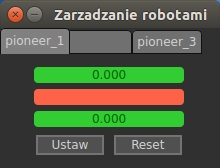
\includegraphics[]{opisy/materialy/zarzadzanie_robotami.jpeg}
 \label{fig:zarzadzanie_robotami}
 \caption{Okno zarz�dzania robotami}
\end{figure}

\subsubsection{Implementacja}
Klasa odpowiadaj�ca za ca�e okienko to \texttt{RobotManagementWindow}. Dziedziczy ona po klasie \texttt{QDialog}. Jej kluczowe metody to:
\begin{lstlisting}[language=C++, numbers=none]
public slots:
	void onAddNewRobot(int id);
	void onHideRobot(int id);
\end{lstlisting}
Odpowiadaj� one za to co dzieje si� w~oknie odpowiednio w~momencie dodania robota i~schowania go. Mianowicie, w~momencie otrzymania odpowiednich sygna��w aktywowana b�d� dezaktywowana jest stosowna zak�adka.

Klasa odpowiadaj�ca za wygl�d zak�adki to \texttt{RobotManagementTab}. Dziedziczy ona po klasie \texttt{QWidget}. Jej kluczowe metody to:
\begin{lstlisting}[language=C++, numbers=none]
void receivedMsg(const boost::shared_ptr<const gazebo::msgs::Int> &msg);
private slots:
	void on_pushButtonUstaw_clicked();
	void on_pushButtonReset_clicked();
\end{lstlisting}














\subsection{Wyniki symulacji}

\bibliographystyle{plabbrv}
\nocite{*}
\bibliography{bibliografia}

\end{document}
